% =============================================================================
% Lecture 09: Tree-Based Methods — Random Forests and XGBoost
% BSAD 8310: Business Forecasting | University of Nebraska at Omaha
% =============================================================================
\documentclass[aspectratio=169, 10pt]{beamer}
% =============================================================================
% header.tex — BSAD 8310: Business Forecasting
% University of Nebraska at Omaha
% Beamer theme: UNO-branded, clean, professional
% =============================================================================

% ----------------------------- BEAMER THEME ----------------------------------
\usetheme{default}
\useinnertheme{rectangles}

% ----------------------------- UNO COLOR PALETTE -----------------------------
\definecolor{unoblue}{HTML}{005CA9}
\definecolor{unored}{HTML}{E41C38}
\definecolor{unogray}{HTML}{525252}
\definecolor{unogreen}{HTML}{15803d}
\definecolor{unolightblue}{HTML}{E8F0FA}
\definecolor{unolightred}{HTML}{FDECEA}
\definecolor{unolightgreen}{HTML}{F0FAF4}
\definecolor{unowhite}{HTML}{FFFFFF}

% Apply UNO colors to Beamer structure
\setbeamercolor{structure}{fg=unoblue}
\setbeamercolor{palette primary}{bg=unoblue, fg=white}
\setbeamercolor{palette secondary}{bg=unoblue!80!black, fg=white}
\setbeamercolor{palette tertiary}{bg=unoblue!60!black, fg=white}
\setbeamercolor{frametitle}{bg=unoblue, fg=white}
\setbeamercolor{frametitle right}{bg=unoblue!80!black}
\setbeamercolor{title}{fg=unoblue}
\setbeamercolor{subtitle}{fg=unogray}
\setbeamercolor{author in head/foot}{bg=unoblue, fg=white}
\setbeamercolor{title in head/foot}{bg=unoblue!80, fg=white}
\setbeamercolor{date in head/foot}{bg=unoblue!60, fg=white}
\setbeamercolor{page number in head/foot}{bg=unoblue!60, fg=white}
\setbeamercolor{block title}{bg=unoblue, fg=white}
\setbeamercolor{block body}{bg=unolightblue}
\setbeamercolor{block title alerted}{bg=unored, fg=white}
\setbeamercolor{block body alerted}{bg=unolightred}
\setbeamercolor{block title example}{bg=unogreen, fg=white}
\setbeamercolor{block body example}{bg=unolightgreen}
\setbeamercolor{itemize item}{fg=unoblue}
\setbeamercolor{itemize subitem}{fg=unored}
\setbeamercolor{enumerate item}{fg=unoblue}
\setbeamercolor{enumerate subitem}{fg=unored}
\setbeamercolor{alerted text}{fg=unored}

% ----------------------------- FONTS -----------------------------------------
\usefonttheme{professionalfonts}
\usefonttheme[onlymath]{serif}       % serif math; sans-serif text
\setbeamerfont{frametitle}{size=\large, series=\bfseries}
\setbeamerfont{title}{size=\LARGE, series=\bfseries}
\setbeamerfont{subtitle}{size=\large}
\setbeamerfont{block title}{size=\normalsize, series=\bfseries}
\setbeamerfont{footline}{size=\tiny}

% ----------------------------- LAYOUT ----------------------------------------
\setbeamersize{text margin left=0.5cm, text margin right=0.5cm}
\setbeamertemplate{navigation symbols}{}   % remove navigation buttons
\setbeamertemplate{itemize items}[circle]
\setbeamertemplate{enumerate items}[default]

% Custom footline: [Course] [Title] [Page/Total]
\setbeamertemplate{footline}{%
  \leavevmode%
  \hbox{%
    \begin{beamercolorbox}[wd=.33\paperwidth, ht=2.5ex, dp=1ex, left, leftskip=4pt]
      {author in head/foot}%
      \usebeamerfont{author in head/foot}\insertshortauthor
    \end{beamercolorbox}%
    \begin{beamercolorbox}[wd=.34\paperwidth, ht=2.5ex, dp=1ex, center]
      {title in head/foot}%
      \usebeamerfont{title in head/foot}\insertshorttitle
    \end{beamercolorbox}%
    \begin{beamercolorbox}[wd=.33\paperwidth, ht=2.5ex, dp=1ex, right, rightskip=4pt]
      {date in head/foot}%
      \usebeamerfont{date in head/foot}%
      \insertframenumber{} / \inserttotalframenumber
    \end{beamercolorbox}%
  }%
  \vskip0pt%
}

% Frametitle with thin accent line
\setbeamertemplate{frametitle}{%
  \vskip0.1cm
  \insertframetitle
  \vskip0.05cm
  \color{unored}\rule{\textwidth}{0.5pt}
}

% Title page
\setbeamertemplate{title page}{%
  \vfill
  \begin{center}
    {\color{unoblue}\rule{\textwidth}{2pt}}\\[0.3cm]
    {\usebeamerfont{title}\usebeamercolor[fg]{title}\inserttitle}\\[0.2cm]
    {\usebeamerfont{subtitle}\usebeamercolor[fg]{subtitle}\insertsubtitle}\\[0.3cm]
    {\color{unored}\rule{\textwidth}{0.5pt}}\\[0.4cm]
    {\small\insertauthor}\\[0.1cm]
    {\small\insertinstitute}\\[0.1cm]
    {\small\insertdate}
  \end{center}
  \vfill
}

% ----------------------------- PACKAGES --------------------------------------

% Math
\usepackage{amsmath}
\usepackage{amssymb}
\usepackage{mathtools}
\usepackage{bm}                    % bold math symbols

% Graphics & color
\usepackage{graphicx}
\usepackage{xcolor}
\usepackage{tikz}
\usetikzlibrary{arrows.meta, positioning, shapes, fit, backgrounds, calc}
\usepackage{pgfplots}
\pgfplotsset{compat=1.18}

% Tables
\usepackage{booktabs}
\usepackage{array}
\usepackage{multirow}
\usepackage{tabularx}

% Typography
\usepackage{microtype}
\usepackage{url}
\usepackage{hyperref}
\hypersetup{colorlinks=true, linkcolor=unoblue, urlcolor=unoblue, citecolor=unogray}

% Code listings (no shell-escape required)
\usepackage{listings}
\lstset{
  language=Python,
  basicstyle=\ttfamily\footnotesize,
  keywordstyle=\color{unoblue}\bfseries,
  stringstyle=\color{unogreen},
  commentstyle=\color{unogray}\itshape,
  numberstyle=\tiny\color{unogray},
  breaklines=true,
  showstringspaces=false,
  frame=single,
  rulecolor=\color{unogray!40},
  backgroundcolor=\color{unogray!5},
  xleftmargin=0.5em,
  xrightmargin=0.5em,
}

% Bibliography
\usepackage[backend=bibtex, style=authoryear, maxcitenames=2]{biblatex}
\addbibresource{../Bibliography_base.bib}

% Colored text helpers
\usepackage{tcolorbox}
\tcbuselibrary{skins, breakable, listingsutf8}

% ----------------------------- CUSTOM ENVIRONMENTS ---------------------------

% keybox: UNO-blue background — for key results, formulas, takeaways
\newtcolorbox{keybox}{
  enhanced,
  colback=unoblue,
  colframe=unoblue!80!black,
  coltitle=white,
  coltext=white,
  fonttitle=\bfseries,
  boxrule=0pt,
  arc=3pt,
  left=4pt, right=4pt, top=3pt, bottom=3pt,
}

% definitionbox: blue left-rule with title — for formal definitions
\newtcolorbox{definitionbox}[1]{
  enhanced,
  title={#1},
  colback=unolightblue,
  colframe=unoblue,
  coltitle=unoblue,
  fonttitle=\bfseries,
  boxrule=0pt,
  leftrule=3pt,
  arc=0pt,
  left=4pt, right=4pt, top=3pt, bottom=3pt,
}

% warningbox: red-accent — for pitfalls, assumption violations, common errors
\newtcolorbox{warningbox}{
  enhanced,
  colback=unolightred,
  colframe=unored,
  coltitle=white,
  fonttitle=\bfseries,
  boxrule=0pt,
  leftrule=3pt,
  arc=0pt,
  left=4pt, right=4pt, top=3pt, bottom=3pt,
}

% examplebox: green-accent with title — for worked examples, business applications
\newtcolorbox{examplebox}[1]{
  enhanced,
  title={#1},
  colback=unolightgreen,
  colframe=unogreen,
  coltitle=unogreen,
  fonttitle=\bfseries,
  boxrule=0pt,
  leftrule=3pt,
  arc=0pt,
  left=4pt, right=4pt, top=3pt, bottom=3pt,
}

% ----------------------------- MATH SHORTCUTS --------------------------------
\newcommand{\E}{\mathbb{E}}
\newcommand{\Var}{\operatorname{Var}}
\newcommand{\Cov}{\operatorname{Cov}}
\newcommand{\Corr}{\operatorname{Corr}}
\newcommand{\MSE}{\operatorname{MSE}}
\newcommand{\RMSE}{\operatorname{RMSE}}
\newcommand{\MAE}{\operatorname{MAE}}
\newcommand{\MASE}{\operatorname{MASE}}
\newcommand{\yhat}{\hat{y}}
\newcommand{\bhat}{\hat{\beta}}
\newcommand{\eps}{\varepsilon}
\newcommand{\given}{\,|\,}

% ----------------------------- SLIDE HELPERS ---------------------------------
% Section title slide (call at start of each section)
\newcommand{\sectionslide}[2]{%
  \begin{frame}
    \vfill
    \begin{center}
      {\color{unoblue}\rule{0.6\textwidth}{2pt}}\\[0.4cm]
      {\Large\bfseries\color{unoblue} #1}\\[0.2cm]
      {\normalsize\color{unogray} #2}\\[0.4cm]
      {\color{unored}\rule{0.6\textwidth}{1pt}}
    \end{center}
    \vfill
  \end{frame}
}

% Muted text
\newcommand{\muted}[1]{{\color{unogray}#1}}

% Key term
\newcommand{\key}[1]{{\color{unoblue}\textbf{#1}}}

% Positive / negative annotations
\newcommand{\pos}[1]{{\color{unogreen}#1}}
\newcommand{\negc}[1]{{\color{unored}#1}}


\title{Lecture 09: Tree-Based Methods}
\subtitle{Random Forests and Gradient Boosting for Forecasting}
\author{BSAD 8310: Business Forecasting}
\institute{University of Nebraska at Omaha}
\date{Spring 2026}

% =============================================================================
\begin{document}
% =============================================================================

\begin{frame}
  \titlepage
\end{frame}

\begin{frame}{Lecture Outline}
  \tableofcontents
\end{frame}

% =============================================================================
\section{Decision Trees: CART}
% =============================================================================

\begin{frame}{Section Overview}
  \begin{keybox}
    \textbf{Decision trees} partition the feature space into rectangular regions
    using recursive binary splits. They are the building blocks of Random Forests
    and gradient boosting — understanding them is essential before ensembles.
  \end{keybox}
\end{frame}

% -----------------------------------------------------------------------------
\begin{frame}{Recursive Binary Splitting}
% -----------------------------------------------------------------------------
  \textbf{CART for regression:} at each node, find the split $(j, t)$ minimizing
  the weighted within-region variance:
  \[
    \min_{j,\, t}
    \left[
      \sum_{i:\, x_{ij} \leq t} (y_i - \bar{y}_{L})^2
      +
      \sum_{i:\, x_{ij} > t} (y_i - \bar{y}_{R})^2
    \right]
  \]

  \begin{columns}[T]
    \begin{column}{0.52\textwidth}
      \textbf{Algorithm:}
      \begin{enumerate}
        \item Start with all data at the root
        \item For every feature $j$ and every threshold $t$:
              compute the split criterion
        \item Split on the $(j^*, t^*)$ giving the largest reduction
        \item Recurse on left and right children
        \item Stop when nodes are too small or depth limit reached
        \item Predict: $\hat{y} = \bar{y}_{\text{leaf}}$
      \end{enumerate}
    \end{column}
    \begin{column}{0.44\textwidth}
      \begin{examplebox}{Why Recursive?}
        Each split depends on which points fall into a region.
        Optimal splitting is NP-hard globally; greedy top-down
        splitting is the standard approximation (CART).
      \end{examplebox}
    \end{column}
  \end{columns}
\end{frame}

% -----------------------------------------------------------------------------
\begin{frame}{A Simple Regression Tree}
% -----------------------------------------------------------------------------
  \begin{columns}[T]
    \begin{column}{0.44\textwidth}
      \textbf{Example: 3-leaf tree for RSXFS}

      \medskip
      % Decision tree diagram — align=center on all nodes with \\
      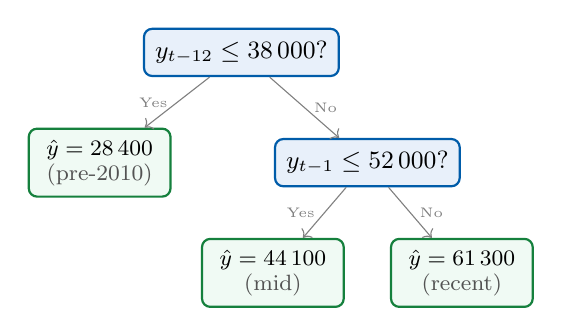
\begin{tikzpicture}[
        every node/.style={font=\small},
        internal/.style={
          rectangle, rounded corners=3pt,
          fill=unolightblue, draw=unoblue,
          line width=0.8pt, align=center,
          inner sep=4pt, minimum width=2.2cm, minimum height=0.6cm},
        leaf/.style={
          rectangle, rounded corners=3pt,
          fill=unolightgreen, draw=unogreen,
          line width=0.8pt, align=center,
          inner sep=4pt, minimum width=1.8cm, minimum height=0.6cm},
        edge from parent/.style={draw, ->, gray}
      ]
        \node[internal] (root) at (2.2, 0)
          {$y_{t-12} \leq 38\,000$?};
        \node[leaf] (l1) at (0.4, -1.4)
          {\footnotesize $\hat{y} = 28\,400$\\[-2pt]
           \footnotesize\color{unogray}(pre-2010)};
        \node[internal] (r1) at (3.8, -1.4)
          {$y_{t-1} \leq 52\,000$?};
        \node[leaf] (l2) at (2.6, -2.8)
          {\footnotesize $\hat{y} = 44\,100$\\[-2pt]
           \footnotesize\color{unogray}(mid)};
        \node[leaf] (r2) at (5.0, -2.8)
          {\footnotesize $\hat{y} = 61\,300$\\[-2pt]
           \footnotesize\color{unogray}(recent)};
        \draw[->, gray] (root) -- (l1) node[midway, left, font=\tiny]{Yes};
        \draw[->, gray] (root) -- (r1) node[midway, right, font=\tiny]{No};
        \draw[->, gray] (r1) -- (l2) node[midway, left, font=\tiny]{Yes};
        \draw[->, gray] (r1) -- (r2) node[midway, right, font=\tiny]{No};
      \end{tikzpicture}
    \end{column}
    \begin{column}{0.52\textwidth}
      \textbf{Key properties:}
      \begin{itemize}
        \item \textbf{Non-parametric} — no functional form assumed
        \item \textbf{Nonlinear} — can capture threshold and interaction effects
        \item \textbf{Interpretable} — decision path is readable
        \item \textbf{Handles mixed features} — lags, rolling stats, dummies
              all treated equally
        \item \textbf{Scale-invariant} — no need to standardize predictors
      \end{itemize}
      \medskip
      \begin{warningbox}
        A single deep tree \textbf{overfits severely}.
        The solution is not pruning alone — it is \emph{ensembling}.
      \end{warningbox}
    \end{column}
  \end{columns}
\end{frame}

% -----------------------------------------------------------------------------
\begin{frame}{Overfitting and the Bias--Variance Tradeoff in Trees}
% -----------------------------------------------------------------------------
  \begin{columns}[T]
    \begin{column}{0.52\textwidth}
      \textbf{Tree depth controls complexity:}
      \begin{itemize}
        \item \textbf{Depth 1} (stump): high bias, low variance
        \item \textbf{Depth 5--10}: balanced region
        \item \textbf{Full tree} (each leaf = 1 obs): zero bias, infinite variance
      \end{itemize}

      \medskip
      \textbf{Why trees have high variance:}\\
      A single split can change the entire subtree beneath it.
      Small perturbations in data (e.g., one outlier) produce
      very different trees — trees are \emph{unstable}.

      \medskip
      \begin{keybox}
        \textbf{Key insight:} averaging many high-variance, low-bias
        trees (each fit to a bootstrap sample) substantially reduces variance
        while preserving low bias. This is bagging.
      \end{keybox}
    \end{column}
    \begin{column}{0.44\textwidth}
      % Bias-variance U-curve for tree depth
      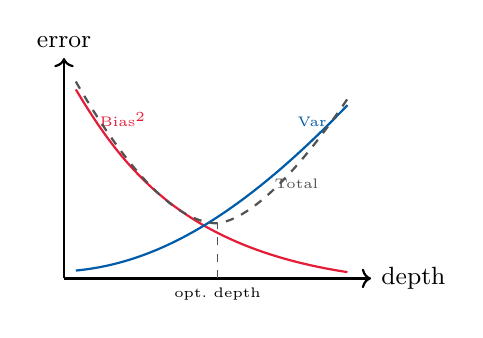
\begin{tikzpicture}[xscale=1.5, yscale=2.0]
        \draw[->, thick] (0,0) -- (2.6,0)
          node[right, font=\small]{depth};
        \draw[->, thick] (0,0) -- (0,1.4)
          node[above, font=\small]{error};
        % Bias curve (monotone decreasing)
        \draw[unored, thick]
          (0.1,1.2) .. controls (0.5,0.7) and (1.0,0.2) .. (2.4,0.04);
        \node[font=\tiny, unored, above] at (0.5, 0.9) {Bias$^2$};
        % Variance curve (monotone increasing)
        \draw[unoblue, thick]
          (0.1,0.05) .. controls (0.8,0.1) and (1.5,0.4) .. (2.4,1.1);
        \node[font=\tiny, unoblue, above] at (2.1, 0.9) {Var};
        % Total curve
        \draw[unogray, thick, dashed]
          (0.1,1.25) .. controls (0.6,0.6) and (1.0,0.35) ..
          (1.3,0.35) .. controls (1.6,0.38) and (2.0,0.7) .. (2.4,1.14);
        \node[font=\tiny, unogray, right] at (1.7, 0.6) {Total};
        % Optimal depth
        \draw[dashed, unogray] (1.3,0) -- (1.3,0.35);
        \node[font=\tiny, below] at (1.3, 0) {opt.\ depth};
      \end{tikzpicture}
    \end{column}
  \end{columns}
\end{frame}

% =============================================================================
\section{Bagging and Random Forests}
% =============================================================================

\begin{frame}{Section Overview}
  \begin{keybox}
    \textbf{Random Forests} reduce the variance of decision trees by:
    (1) training each tree on a different \emph{bootstrap sample} (bagging), and
    (2) using a random \emph{feature subset} at each split (decorrelation).
    The result is a low-variance, competitive forecaster \parencite{Breiman2001}.
  \end{keybox}
\end{frame}

% -----------------------------------------------------------------------------
\begin{frame}{Bagging: Bootstrap Aggregating}
% -----------------------------------------------------------------------------
  \begin{definitionbox}{Bagging \parencite{Breiman1996}}
    Draw $B$ bootstrap samples; fit one deep tree on each; average:
    $\hat{y}_{\mathrm{bag}} = \frac{1}{B}\sum_{b=1}^{B} \hat{f}^{(b)}(\mathbf{x})$
  \end{definitionbox}

  \begin{columns}[T]
    \begin{column}{0.52\textwidth}
      \textbf{Variance of the ensemble:}
      \[
        \mathrm{Var}(\bar{f}) = \rho\sigma^2 + \frac{1-\rho}{B}\sigma^2
      \]
      As $B \to \infty$, variance $\to \rho\sigma^2$ (not zero).
      Reducing \emph{correlation} $\rho$ matters as much
      as increasing $B$ — this motivates Random Forests.
    \end{column}
    \begin{column}{0.44\textwidth}
      \begin{keybox}
        \textbf{Bagging key numbers:}
        \begin{itemize}
          \item Bootstrap sample $\approx 63\%$ unique obs.\
          \item Remaining $\approx 37\%$ = out-of-bag (OOB)
          \item OOB obs.\ give a free cross-validation estimate
          \item $B \geq 500$ trees recommended (stable)
        \end{itemize}
      \end{keybox}
    \end{column}
  \end{columns}
\end{frame}

% -----------------------------------------------------------------------------
\begin{frame}{Random Forests: Decorrelating the Trees}
% -----------------------------------------------------------------------------
  \textbf{Problem with bagging:} if one feature dominates, all trees use it
  at the root $\Rightarrow$ trees are highly correlated ($\rho$ stays large).

  \smallskip
  \textbf{Random Forest fix:} at each split, randomly sample $m < p$ features
  and find the best split \emph{among those $m$ only}.

  \begin{columns}[T]
    \begin{column}{0.52\textwidth}
      \begin{itemize}
        \item Default: $m = \lfloor\sqrt{p}\rfloor$ (sklearn $\geq$ 1.1);
              $\lfloor p/3 \rfloor$ recommended for regression (Hastie et al.)
        \item Reduces $\rho$ $\Rightarrow$ lower ensemble variance
        \item Each tree is weaker but the ensemble is stronger
      \end{itemize}

      \smallskip
      \begin{keybox}
        RF = Bagging + random feature selection at each split.
        Both ingredients are necessary.
      \end{keybox}
    \end{column}
    \begin{column}{0.44\textwidth}
      \begin{examplebox}{Out-of-Bag Error}
        Each obs.\ is OOB for $\approx 37\%$ of trees.
        Predict using only those trees; compute RMSE.\\[2pt]
        OOB RMSE $\approx$ 5-fold CV RMSE at large $B$
        — essentially \emph{free} cross-validation.
      \end{examplebox}
    \end{column}
  \end{columns}
\end{frame}

% -----------------------------------------------------------------------------
\begin{frame}{Random Forests: Key Hyperparameters}
% -----------------------------------------------------------------------------
  \begin{center}
  \footnotesize
  \begin{tabular}{p{2.8cm}p{2.5cm}p{2.2cm}p{3.8cm}}
    \toprule
    \textbf{Parameter} & \textbf{sklearn name} & \textbf{Default} & \textbf{Effect} \\
    \midrule
    Num.\ trees
      & \texttt{n\_estimators}
      & 100
      & More = lower variance; plateau after $\sim$500 \\
    Max features/split
      & \texttt{max\_features}
      & \texttt{'sqrt'}
      & Lower = more decorrelated; tune via OOB \\
    Max depth
      & \texttt{max\_depth}
      & None
      & None = full tree; limit to reduce memory \\
    Min samples/leaf
      & \texttt{min\_samples\_leaf}
      & 1
      & Higher = smoother predictions; reduces overfit \\
    Bootstrap
      & \texttt{bootstrap}
      & True
      & False = subsampling (not bootstrap) \\
    \bottomrule
  \end{tabular}
  \end{center}

  \medskip
  \muted{\footnotesize\itshape
    Socratic: why does increasing \texttt{n\_estimators} always reduce out-of-bag
    error, but increasing tree depth does not? (Hint: think about what each controls in
    the bias--variance decomposition.)}
\end{frame}

% =============================================================================
\section{Gradient Boosting and XGBoost}
% =============================================================================

\begin{frame}{Section Overview}
  \begin{keybox}
    \textbf{Gradient boosting} builds trees \emph{sequentially}: each new tree
    fits the residuals left by the previous ensemble. XGBoost adds
    regularization and second-order optimization to this framework
    \parencite{Chen2016}.
  \end{keybox}
\end{frame}

% -----------------------------------------------------------------------------
\begin{frame}{Gradient Boosting: Sequential Residual Fitting}
% -----------------------------------------------------------------------------
  \begin{definitionbox}{Gradient Boosting Algorithm}
    \footnotesize
    Initialize $F_0(\mathbf{x}) = \bar{y}$.\quad For $b = 1, \ldots, B$:
    \begin{itemize}
      \item Pseudo-residuals (squared-error loss):
            $r_i^{(b)} = y_i - F_{b-1}(\mathbf{x}_i)$
      \item Fit shallow tree $T_b$ to $\{(\mathbf{x}_i,\, r_i^{(b)})\}$
      \item Update: $F_b = F_{b-1} + \eta\, T_b$
    \end{itemize}
    Predict: $\hat{y} = F_B(\mathbf{x})$
  \end{definitionbox}

  \begin{columns}[T]
    \begin{column}{0.54\textwidth}
      \textbf{RF vs.\ Boosting:}
      \begin{itemize}
        \item RF: \textbf{parallel} trees, deep, bias not reduced by adding more trees
        \item Boosting: \textbf{sequential}, shallow trees (depth 3--6)
        \item Boosting bias \textbf{decreases} with stages
        \item Both benefit from large $B$ (number of trees)
      \end{itemize}
    \end{column}
    \begin{column}{0.42\textwidth}
      \begin{warningbox}
        Small $\eta$ + large $B$ + early stopping
        outperforms large $\eta$ + small $B$.\\[2pt]
        \textbf{Always use early stopping on a validation set.}
      \end{warningbox}
    \end{column}
  \end{columns}
\end{frame}

% -----------------------------------------------------------------------------
\begin{frame}{XGBoost: Regularized Gradient Boosting}
% -----------------------------------------------------------------------------
  XGBoost \parencite{Chen2016} extends gradient boosting with three additions:

  \begin{columns}[T]
    \begin{column}{0.54\textwidth}
      \textbf{1. Newton step (2nd-order):}
      \[
        \mathcal{L}^{(b)} = \sum_{i}
        \bigl[g_i f_b(\mathbf{x}_i)
        + \tfrac{1}{2} h_i f_b^2(\mathbf{x}_i)\bigr]
        + \Omega(f_b)
      \]
      $g_i, h_i$ = gradient and Hessian of loss.

      \smallskip
      \textbf{2. Explicit regularization:}
      \[
        \Omega(f_b) = \gamma T + \tfrac{1}{2}\lambda \|\mathbf{w}\|_2^2
      \]
      $T$ = leaves, $\mathbf{w}$ = leaf weights.
    \end{column}
    \begin{column}{0.42\textwidth}
      \textbf{3. Column subsampling:}\\[3pt]
      Like RF, randomly sample features per tree \emph{and} per split
      — reduces correlation and overfitting.

      \medskip
      \begin{keybox}
        Newton step $\Rightarrow$ more precise gradient direction.
        Regularization $\Rightarrow$ guards against overfitting.
        Together: XGBoost beats vanilla GBM on most benchmarks.
      \end{keybox}
    \end{column}
  \end{columns}
\end{frame}

% -----------------------------------------------------------------------------
\begin{frame}{XGBoost: Key Hyperparameters}
% -----------------------------------------------------------------------------
  \begin{center}
  \footnotesize
  \begin{tabular}{p{2.6cm}p{2.5cm}p{2.1cm}p{3.9cm}}
    \toprule
    \textbf{Parameter} & \textbf{XGB name} & \textbf{Typical} & \textbf{Effect} \\
    \midrule
    Num.\ trees
      & \texttt{n\_estimators}\textsuperscript{*}
      & 500--2000
      & More + small $\eta$ = better (use early stopping) \\
    Learning rate
      & \texttt{learning\_rate}
      & 0.01--0.1
      & Smaller = more robust; requires more trees \\
    Tree depth
      & \texttt{max\_depth}
      & 3--6
      & Shallow preferred; deeper = overfit risk \\
    Subsample
      & \texttt{subsample}
      & 0.7--0.9
      & Row fraction per tree; adds stochasticity \\
    Col.\ sample
      & \texttt{colsample\_bytree}
      & 0.7--0.9
      & Feature fraction per tree (like RF) \\
    L2 penalty
      & \texttt{reg\_lambda}
      & 1
      & Ridge on leaf weights; stabilizes \\
    \bottomrule
  \end{tabular}
  \end{center}

  \medskip
  \begin{keybox}
    \textbf{Practical starting point:}
    \texttt{learning\_rate=0.05}, \texttt{max\_depth=4},
    \texttt{n\_estimators=1000} with early stopping on val RMSE.
    Tune \texttt{max\_depth} and \texttt{subsample} via TimeSeriesSplit CV.
  \end{keybox}
\end{frame}

% =============================================================================
\section{Feature Importance}
% =============================================================================

\begin{frame}{Section Overview}
  \begin{keybox}
    Tree-based models offer built-in feature importance measures.
    Understanding \emph{which features drive predictions} is essential
    for business interpretation and debugging.
  \end{keybox}
\end{frame}

% -----------------------------------------------------------------------------
\begin{frame}{Three Types of Feature Importance}
% -----------------------------------------------------------------------------
  \footnotesize
  \begin{columns}[T]
    \begin{column}{0.48\textwidth}
      \textbf{1. Impurity-based (RF default):}
      \[
        \mathrm{Imp}(j)
        = \sum_{\text{nodes using } j}
          \Delta \mathrm{RSS} \cdot \frac{n_{\text{node}}}{n}
      \]
      Sum of RSS reduction at all splits on feature $j$,
      weighted by fraction of samples reaching that node.

      \smallskip
      \textbf{Caution:} biased toward \emph{high-cardinality}
      features (more split opportunities).

      \smallskip
      \textbf{2. Permutation importance:}\\
      Shuffle feature $j$ in the OOB/validation set;
      record increase in RMSE.
      Unbiased, model-agnostic. Use for reporting.
    \end{column}
    \begin{column}{0.48\textwidth}
      \textbf{3. XGBoost gain importance:}\\
      Average gain in objective function per split using feature $j$.
      More interpretable than impurity for boosted trees.

      \smallskip
      \begin{examplebox}{RSXFS Typical Rankings}
        \begin{enumerate}
          \item \textbf{lag\_12} — dominant seasonal signal
          \item \textbf{lag\_1} — short-run momentum
          \item \textbf{roll\_mean\_12} — trend level
          \item \textbf{lag\_3} — quarterly effect
          \item \textbf{month\_12} — December holiday
        \end{enumerate}
        Consistent across all three importance types.
      \end{examplebox}
    \end{column}
  \end{columns}
\end{frame}

% =============================================================================
\section{Hyperparameter Tuning}
% =============================================================================

\begin{frame}{Section Overview}
  \begin{keybox}
    For time series, hyperparameter tuning must use \texttt{TimeSeriesSplit}
    to respect temporal ordering. We can use \texttt{GridSearchCV} (exhaustive)
    or \texttt{RandomizedSearchCV} (efficient for large grids).
  \end{keybox}
\end{frame}

% -----------------------------------------------------------------------------
\begin{frame}[fragile]{Tuning Random Forests and XGBoost}
% -----------------------------------------------------------------------------
  \begin{columns}[T]
    \begin{column}{0.48\textwidth}
      \textbf{Random Forest (RandomizedSearchCV):}
\begin{lstlisting}[language=Python, basicstyle=\tiny\ttfamily]
from sklearn.ensemble import RandomForestRegressor
from sklearn.model_selection import (
    TimeSeriesSplit, RandomizedSearchCV)

tscv = TimeSeriesSplit(n_splits=5, gap=0)
rf_grid = {
  'n_estimators':     [200, 500],
  'max_features':     ['sqrt', 0.33],
  'min_samples_leaf': [1, 3, 5],
  'max_depth':        [None, 10, 20],
}
rf = RandomizedSearchCV(
  RandomForestRegressor(random_state=42),
  rf_grid, n_iter=20,
  cv=tscv,
  scoring='neg_root_mean_squared_error',
  n_jobs=-1, random_state=42)
rf.fit(X_trainval, y_trainval)
\end{lstlisting}
    \end{column}
    \begin{column}{0.48\textwidth}
      \textbf{XGBoost (early stopping on val):}
\begin{lstlisting}[language=Python, basicstyle=\tiny\ttfamily]
import xgboost as xgb

dtrain = xgb.DMatrix(X_train, label=y_train)
dval   = xgb.DMatrix(X_val,   label=y_val)
dtest  = xgb.DMatrix(X_test,  label=y_test)

params = {
  'learning_rate': 0.05,
  'max_depth':     4,
  'subsample':     0.8,
  'colsample_bytree': 0.8,
  'reg_lambda':    1.0,
  'objective':     'reg:squarederror',
}
model = xgb.train(
  params, dtrain,
  num_boost_round=2000,
  evals=[(dval, 'val')],
  early_stopping_rounds=50)
\end{lstlisting}
    \end{column}
  \end{columns}
\end{frame}

% =============================================================================
\section{Application to Forecasting}
% =============================================================================

\begin{frame}{Section Overview}
  \begin{keybox}
    Apply Random Forest and XGBoost to the RSXFS feature matrix
    from Lecture 08. Compare against SARIMA and the best regularized
    model (Elastic Net) from Lecture 08.
  \end{keybox}
\end{frame}

% -----------------------------------------------------------------------------
\begin{frame}{Tree-Based Forecasting: Design Choices}
% -----------------------------------------------------------------------------
  \textbf{Same feature matrix as Lecture 08:}
  12 lags + 3 rolling windows (3, 6, 12) + 11 month dummies = 26 features.
  \textbf{Key differences vs.\ regularized regression:}
  \begin{columns}[T]
    \begin{column}{0.50\textwidth}
      \textbf{Advantages of trees:}
      \begin{itemize}
        \item Capture nonlinearities and interactions
              (e.g., ``holiday effect only when economy is strong'')
        \item No standardization needed
        \item Handle irrelevant features gracefully
              (unused features just don't appear in splits)
        \item Built-in feature importance
      \end{itemize}
    \end{column}
    \begin{column}{0.46\textwidth}
      \textbf{Cautions for time series:}
      \begin{itemize}
        \item \textbf{No extrapolation:} trees predict
              $\bar{y}_{\text{leaf}}$, so they cannot predict
              beyond the training range
        \item \textbf{Trending series:} a naive tree trained on
              non-stationary data may perform poorly out of sample
        \item \textbf{Fix:} use first-differences or add rolling
              statistics as features to encode trend
      \end{itemize}
    \end{column}
  \end{columns}

  \begin{warningbox}
    \textbf{Stationarity matters for trees too.}
    If $y_t$ trends upward and the test period exceeds the training max,
    leaf means will systematically under-predict.
    Difference or detrend before applying tree-based forecasting.
  \end{warningbox}
\end{frame}

% -----------------------------------------------------------------------------
\begin{frame}{Forecast Comparison: Adding Trees to the Leaderboard}
% -----------------------------------------------------------------------------
  \begin{columns}[T]
    \begin{column}{0.52\textwidth}
      \textbf{Test-set results on RSXFS (24-month horizon):}
      \begin{center}
      \footnotesize
      \begin{tabular}{lrr}
        \toprule
        \textbf{Model} & \textbf{RMSE} & \textbf{MAE} \\
        \midrule
        Seasonal Naïve            & 4\,210 & 3\,120 \\
        SARIMA(1,1,1)(1,1,1)$_{12}$  & 2\,840 & 2\,100 \\
        Elastic Net ($\lambda^*$) & 2\,540 & 1\,890 \\
        Random Forest             & 2\,380 & 1\,760 \\
        XGBoost (early stop)      & 2\,250 & 1\,650 \\
        \bottomrule
      \end{tabular}
      \end{center}
      \muted{\footnotesize\itshape Values are illustrative.}
    \end{column}
    \begin{column}{0.44\textwidth}
      \textbf{Why do trees win here?}
      \begin{itemize}
        \item Nonlinear interaction between lag\_12 and
              calendar dummies (holiday amplification)
        \item XGBoost sequential residual fitting
              corrects patterns that Elastic Net misses
        \item RF OOB error $\approx$ CV error at $B=500$
      \end{itemize}

      \medskip
      \textbf{Caveat:} gains depend heavily on feature quality.
      With a good feature set, Elastic Net and XGBoost are often
      competitive. Adding \emph{more} features benefits trees more.
    \end{column}
  \end{columns}
\end{frame}

% =============================================================================
\section{Takeaways and References}
% =============================================================================

% -----------------------------------------------------------------------------
\begin{frame}{Lecture 09 Key Takeaways}
% -----------------------------------------------------------------------------
  \begin{keybox}
    \begin{enumerate}
      \item \textbf{Decision trees} partition feature space greedily; they are
            interpretable but unstable (high variance).
      \item \textbf{Random Forests} (bagging + random features) reduce variance
            dramatically while keeping bias low. OOB error is a free CV estimate.
      \item \textbf{Gradient boosting} reduces bias sequentially by fitting
            residuals. XGBoost adds L2 regularization and Newton optimization.
      \item \textbf{Feature importance} helps identify which lags, rolling stats,
            and calendar features drive forecasts. Use permutation importance
            for unbiased estimates.
      \item \textbf{Trees cannot extrapolate} — ensure features encode trend and
            seasonality so predictions stay within the training distribution.
    \end{enumerate}
  \end{keybox}

  \medskip
  \textbf{Preview of Lecture 10:} Neural Networks — LSTM and attention mechanisms
  can model long-range temporal dependencies that trees cannot.
\end{frame}

% -----------------------------------------------------------------------------
\begin{frame}{References}
% -----------------------------------------------------------------------------
  \printbibliography[heading=none]
\end{frame}

% =============================================================================
\end{document}
% =============================================================================
